\providecommand{\main}{../../../..}
\documentclass[\main/dresen_thesis.tex]{subfiles}
\begin{document}
  \label{sec:looselyPackedNS:bilayerStacks:pnr}

  \begin{figure}[tb]
    \centering
    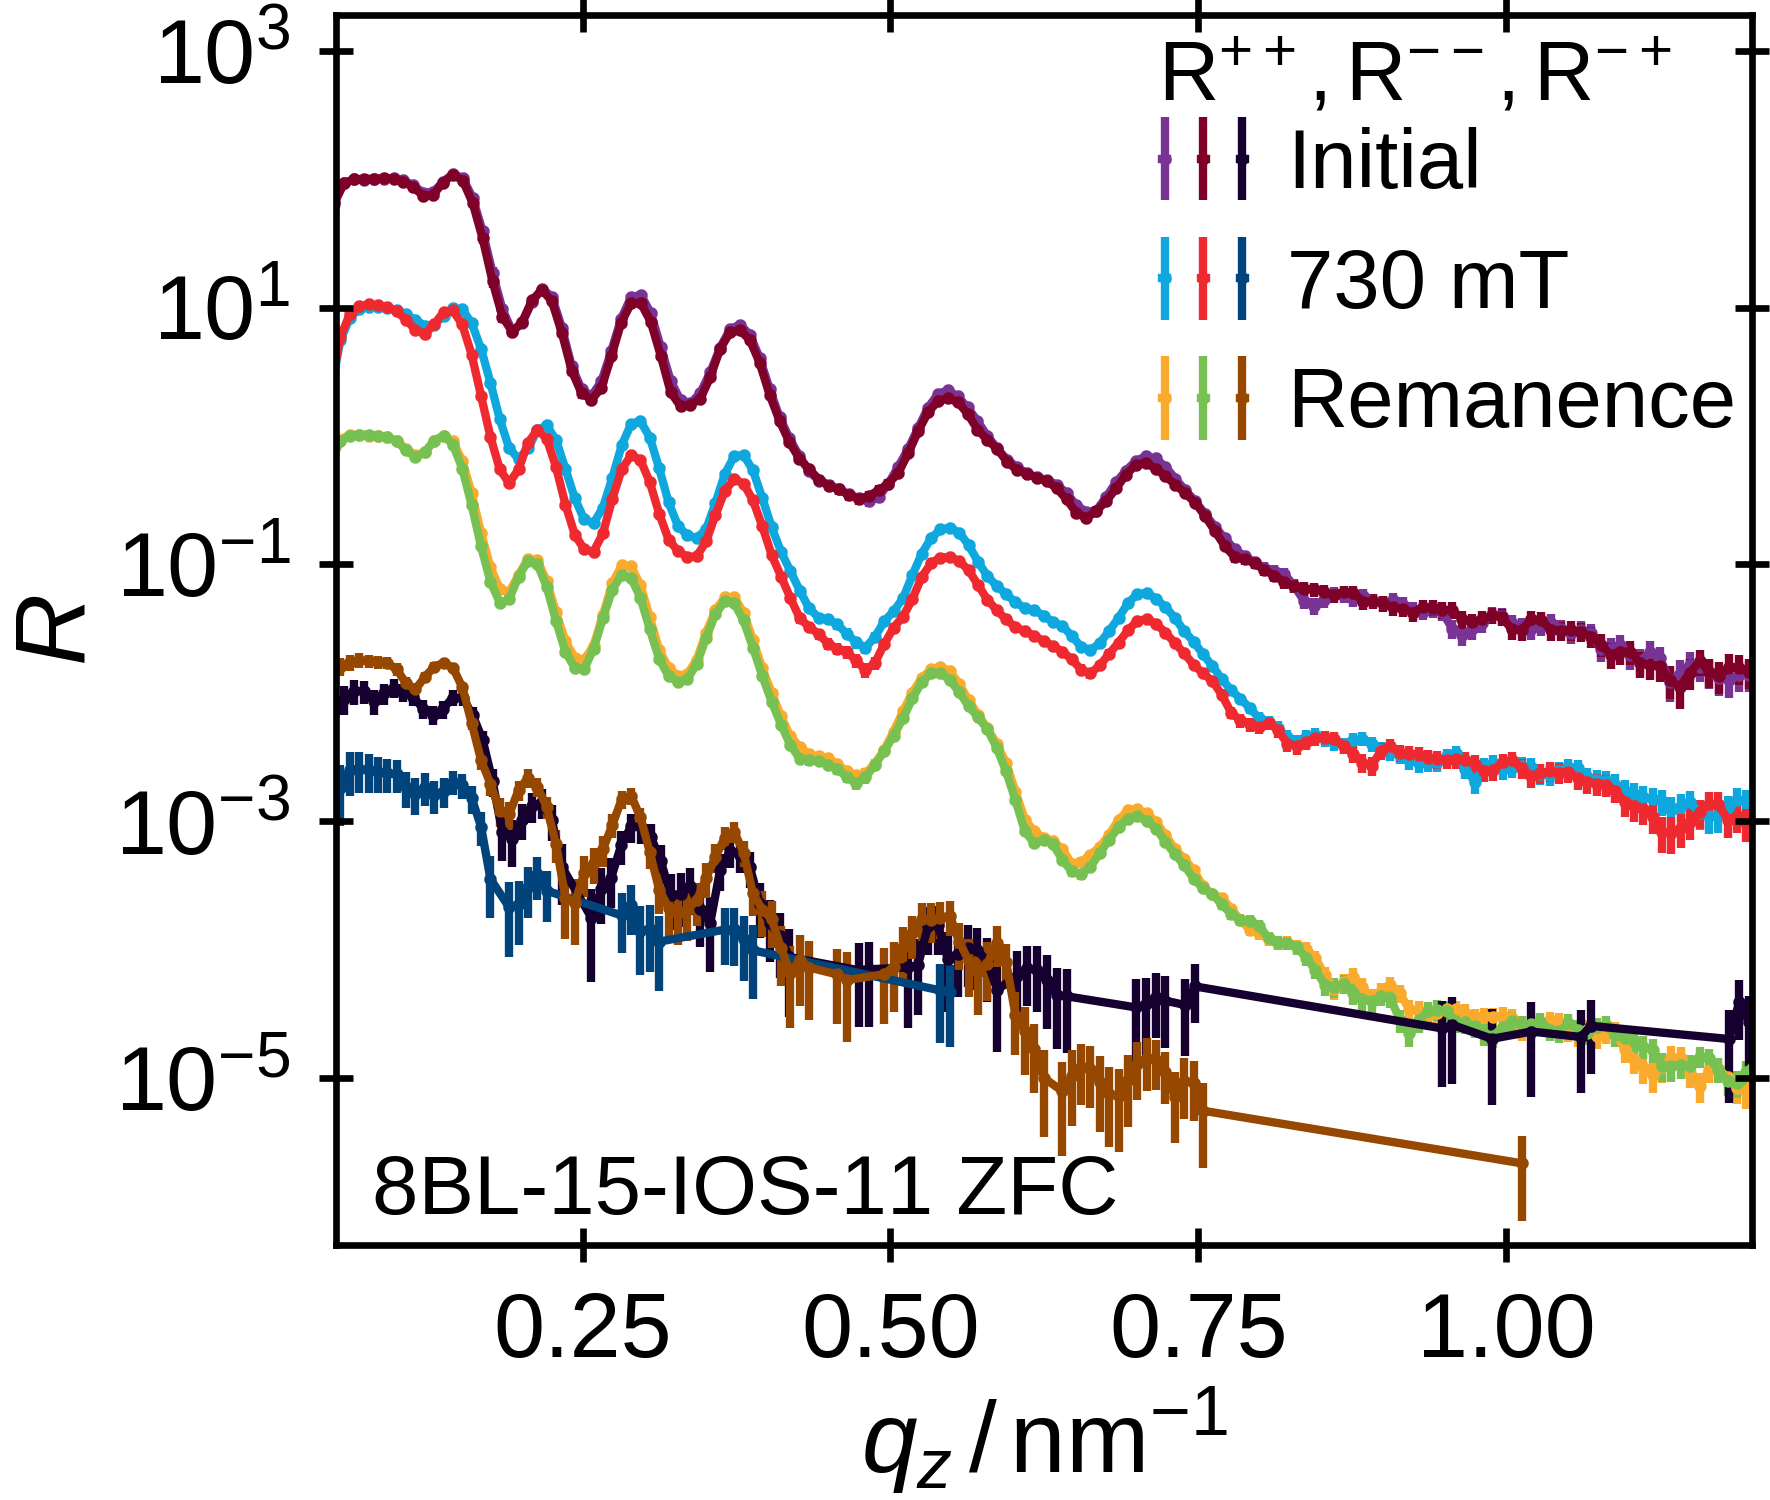
\includegraphics{looselyPackedNP_VerticalStructure_8BL-15-IOS-11_PNR_ZFC30K}
    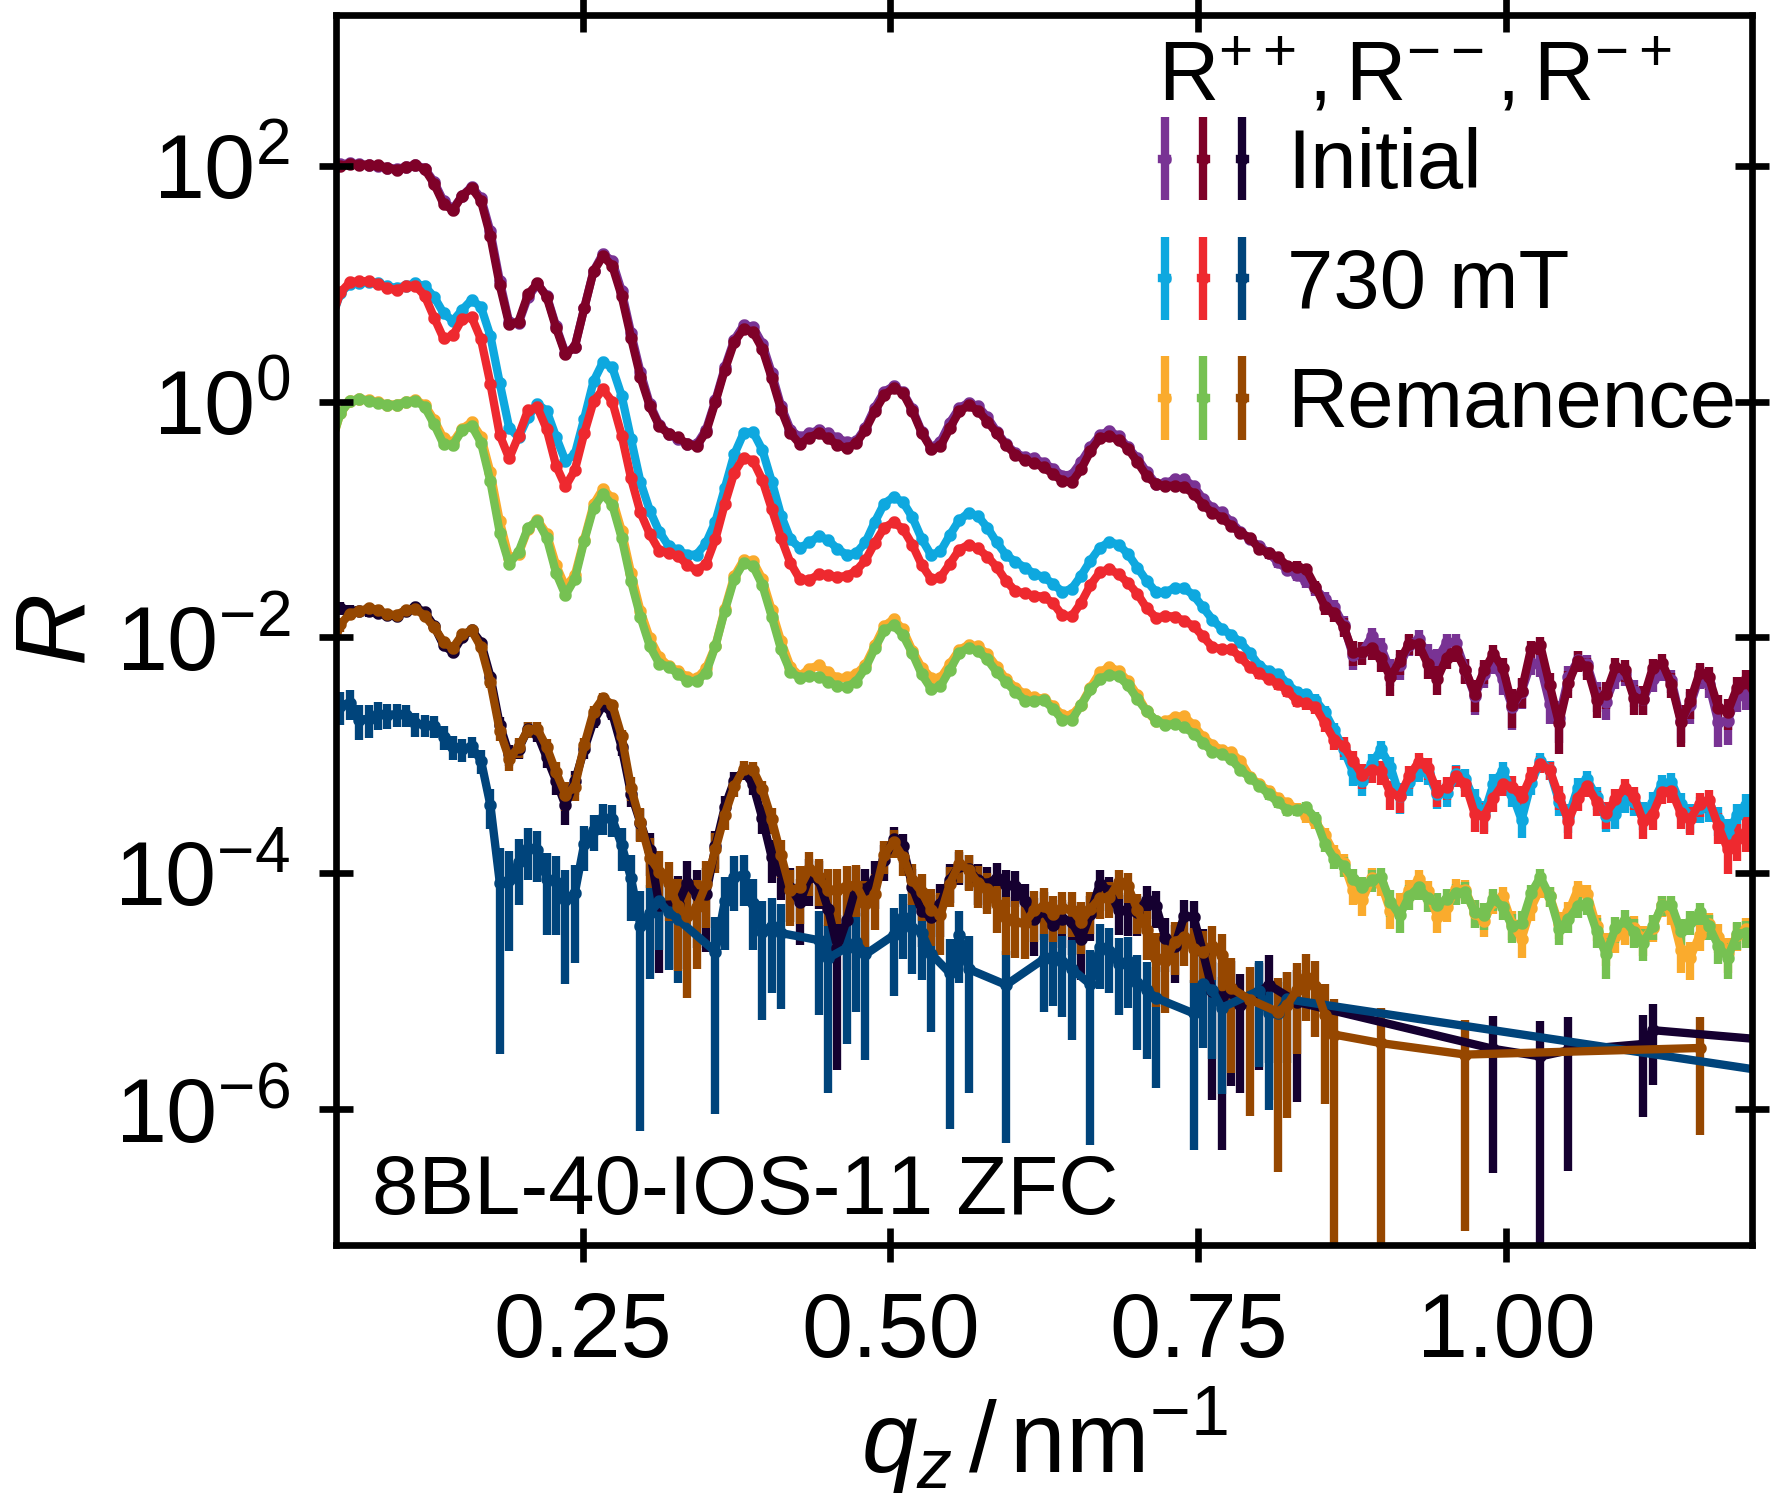
\includegraphics{looselyPackedNP_VerticalStructure_8BL-40-IOS-11_PNR_ZFC30K}
    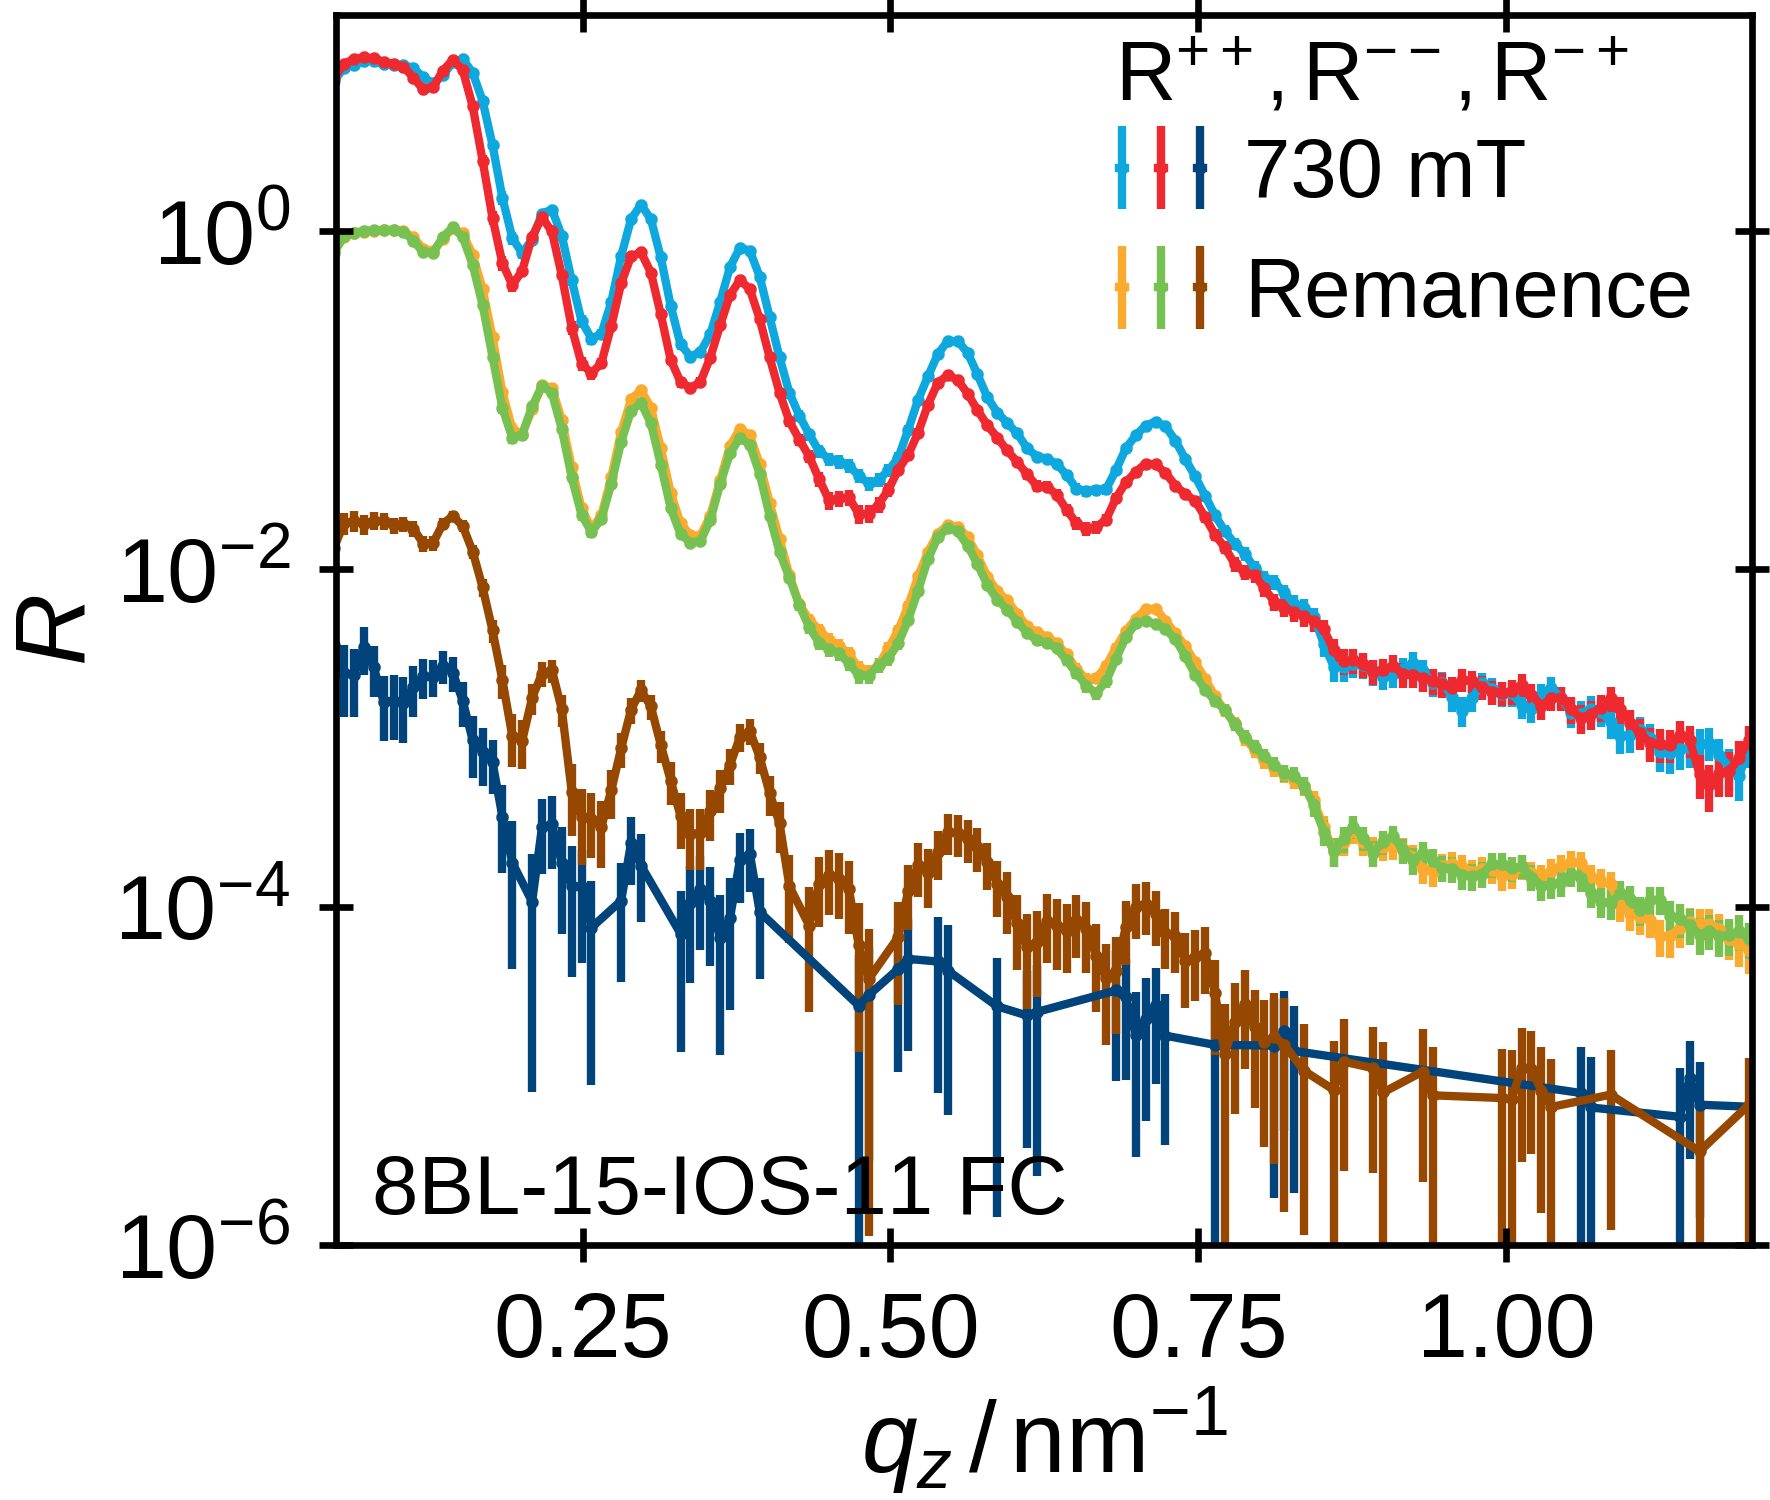
\includegraphics{looselyPackedNP_VerticalStructure_8BL-15-IOS-11_PNR_FC30K}
    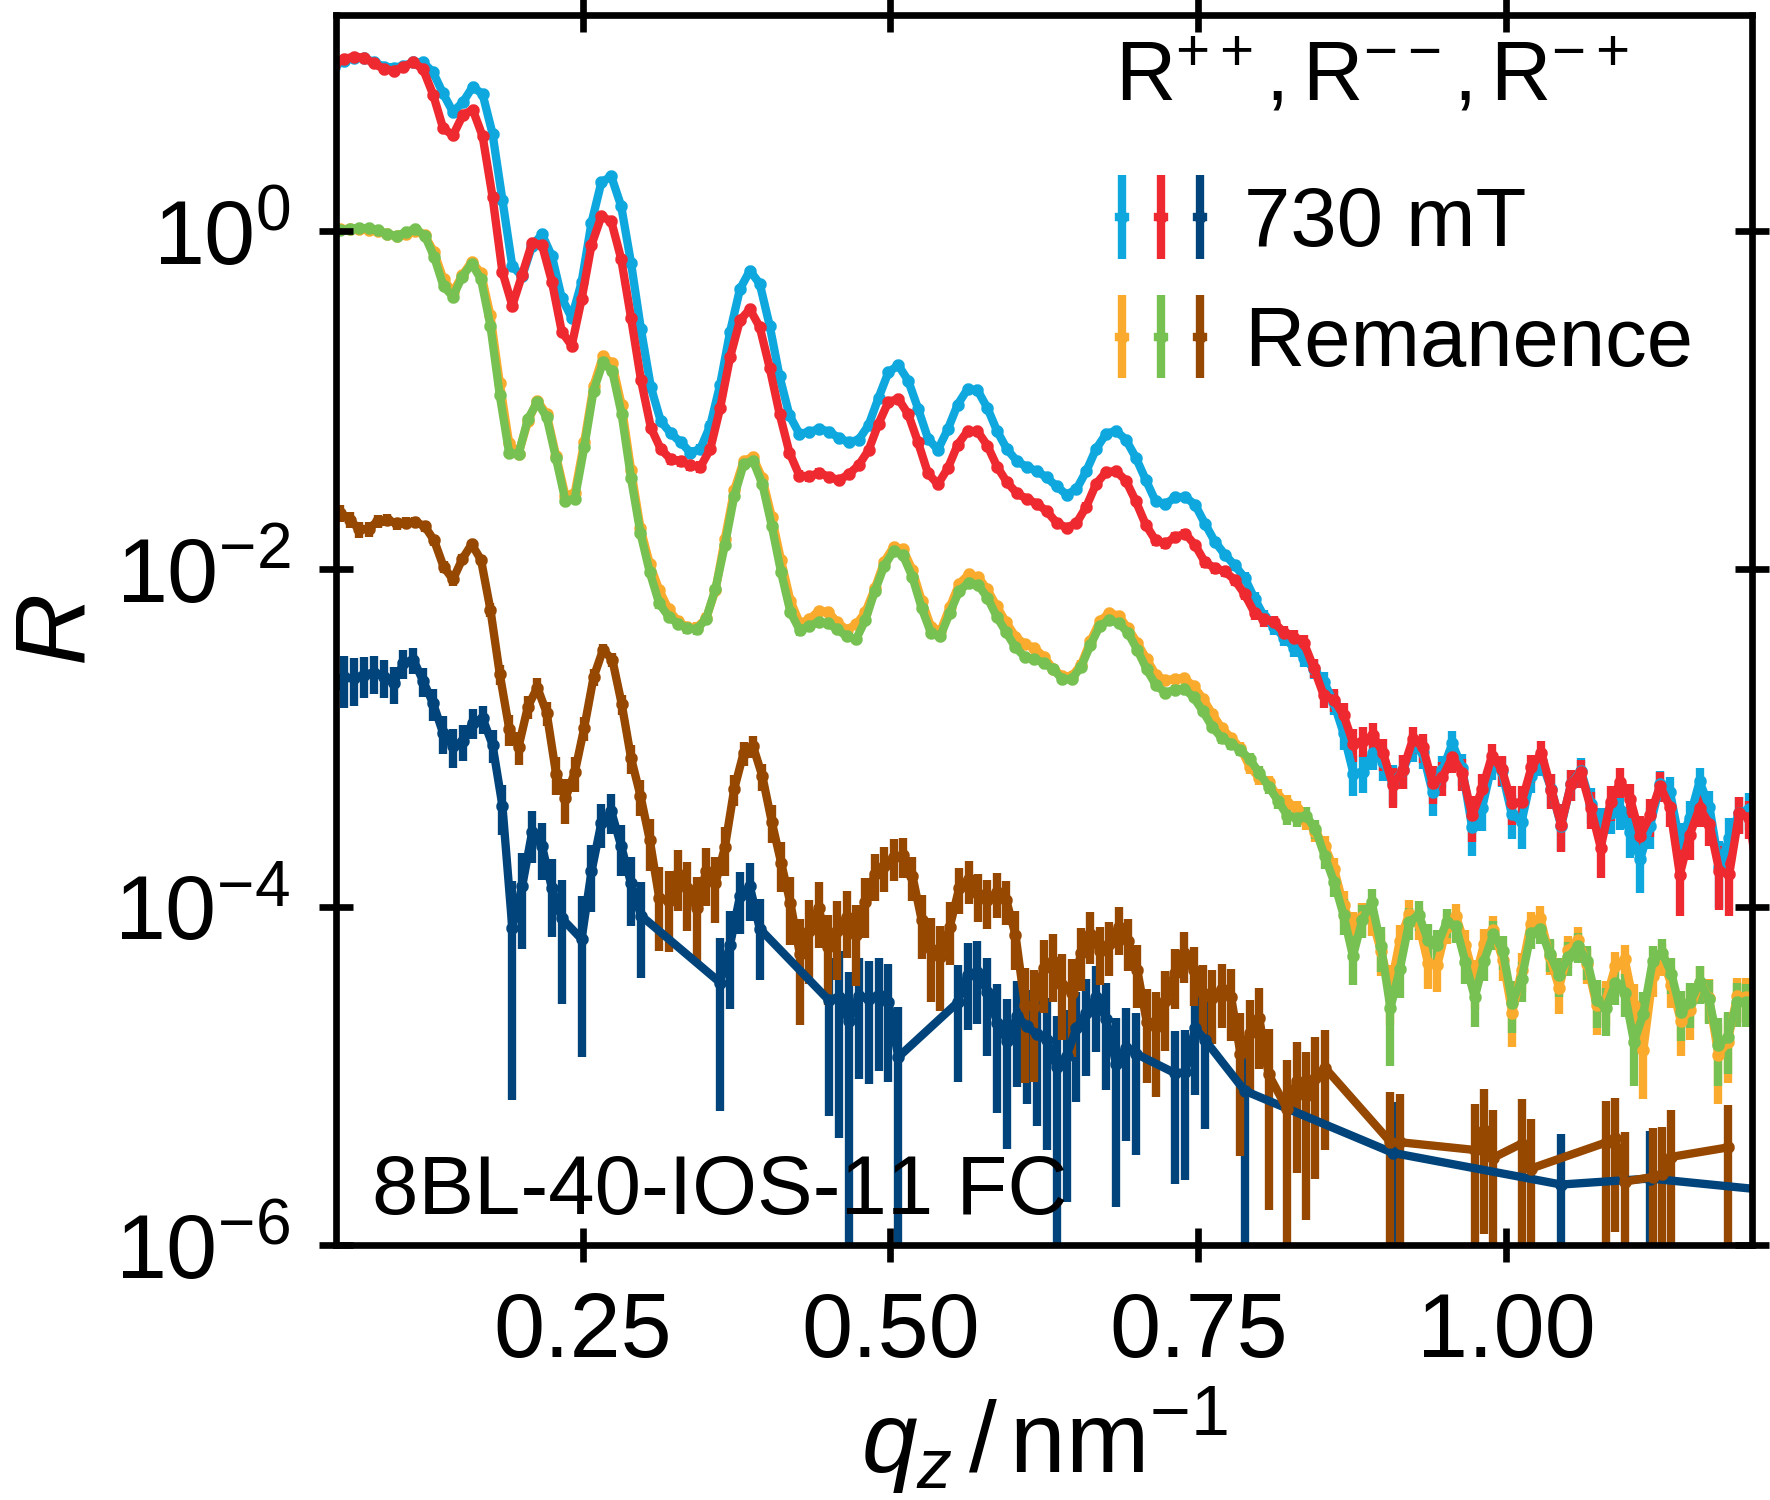
\includegraphics{looselyPackedNP_VerticalStructure_8BL-40-IOS-11_PNR_FC30K}
    \caption{\label{fig:looselyPackedNP:bilayer:pnr:8BL-x-IOS11}Polarized neutron reflectometry with polarization analysis for 8BL-15-IOS-11 (left) and 8BL-40-IOS-11 (right) after zero-field cooling (upper) and field cooling (lower). The non-spin flip reflectivities are scaled by factors of ten for better visibility. }
  \end{figure}

  Analogue to the single layer of spin-coated nanospheres in \refsec{sec:looselyPackedNS:layers:pnr}, the bilayer stacks have been extensively measured at SuperADAM (\refsec{ch:lss:superadam}) at room temperature and at a low temperature of $30 \unit{K}$ for the study of their magnetic properties.
  As no nuclear scattering length density profile could be fit to the non-magnetized samples, the magnetic scattering length density profile can also not be discussed in a quantitative manner and therefore the following discussion of the data is on a qualitative level.

  For the samples 8BL-x-IOS-11, polarized neutron reflectivity with polarization analysis has been performed to study whether contributions in the spin-flip channel are observable.
  The non-spin-flip and spin-flip reflectivities of 8BL-15-IOS-11 are shown in \reffig{fig:looselyPackedNP:bilayer:pnr:8BL-x-IOS11}, after field cooling and zero-field cooling.
  In both cases, a splitting for the reflectivities $R^{++}$ and $R^{--}$ is visible upon magnetization of the sample, which after removal of the magnetic field is no longer visible in the remanent state.
  No additional structure is observed in the polarized channels, as to why it can be assumed that the sample is homogeneously magnetized and no strong antiferromagnetic coupling between the layers is present.

  The reflectivity in the spin-flip channels are in all cases on the order of the polarization efficiency and can be attributed as result of the $1 - 2 \%$ spin-leakage from the non-spin flip channels.
  The absence of spin-flip scattering in all cases suggests that the samples are magnetized for most parts collinear to the magnetizing field.
  The observations are parallel to the results obtained for the single-layer of loosely packed nanospheres in \refsec{sec:looselyPackedNS:layers:pnr}.
  For the sample 8BL-40-IOS-11, with the larger PMMA thickness, the same qualitative observations are made in all cases as shown in \reffig{fig:looselyPackedNP:bilayer:pnr:8BL-x-IOS11}.

  The bilayer stack samples 8BL-x-IOS-7, shown in \reffig{fig:looselyPackedNP:bilayer:pnr:8BL-x-IOS7}, were measured without polarization analysis to improve the counting statistics in $R^{+}$ and $R^{-}$.
  In comparison to the weak splitting of the reflectivity channels $R^{+}$ and $R^{-}$ observed for the single-layer of loosely packed nanospheres SC-IOS-7 at $730 \unit{mT}$ in \refsec{sec:looselyPackedNS:layers:pnr}, the bilayer stacks show a well visible splitting of the polarization channels in the magnetized state.
  However, similar to the bilayer stack samples from IOS-11, no contrast or additional structure are visible in the magnetized or remanent state, neither after the field-cooling experiments nor after the zero-field cooling procedure.
  Thus, it can be concluded that the sample is to large parts homogeneously magnetized across the layers and on average no strong coupling effects are observed.
  The study of weak interaction effects in the sample are inaccessible due to the complex sample structure and the large number of unknown geometrical parameters that are needed for a thorough analysis of the polarized neutron reflectivity data.

  \begin{figure}[tb]
    \centering
    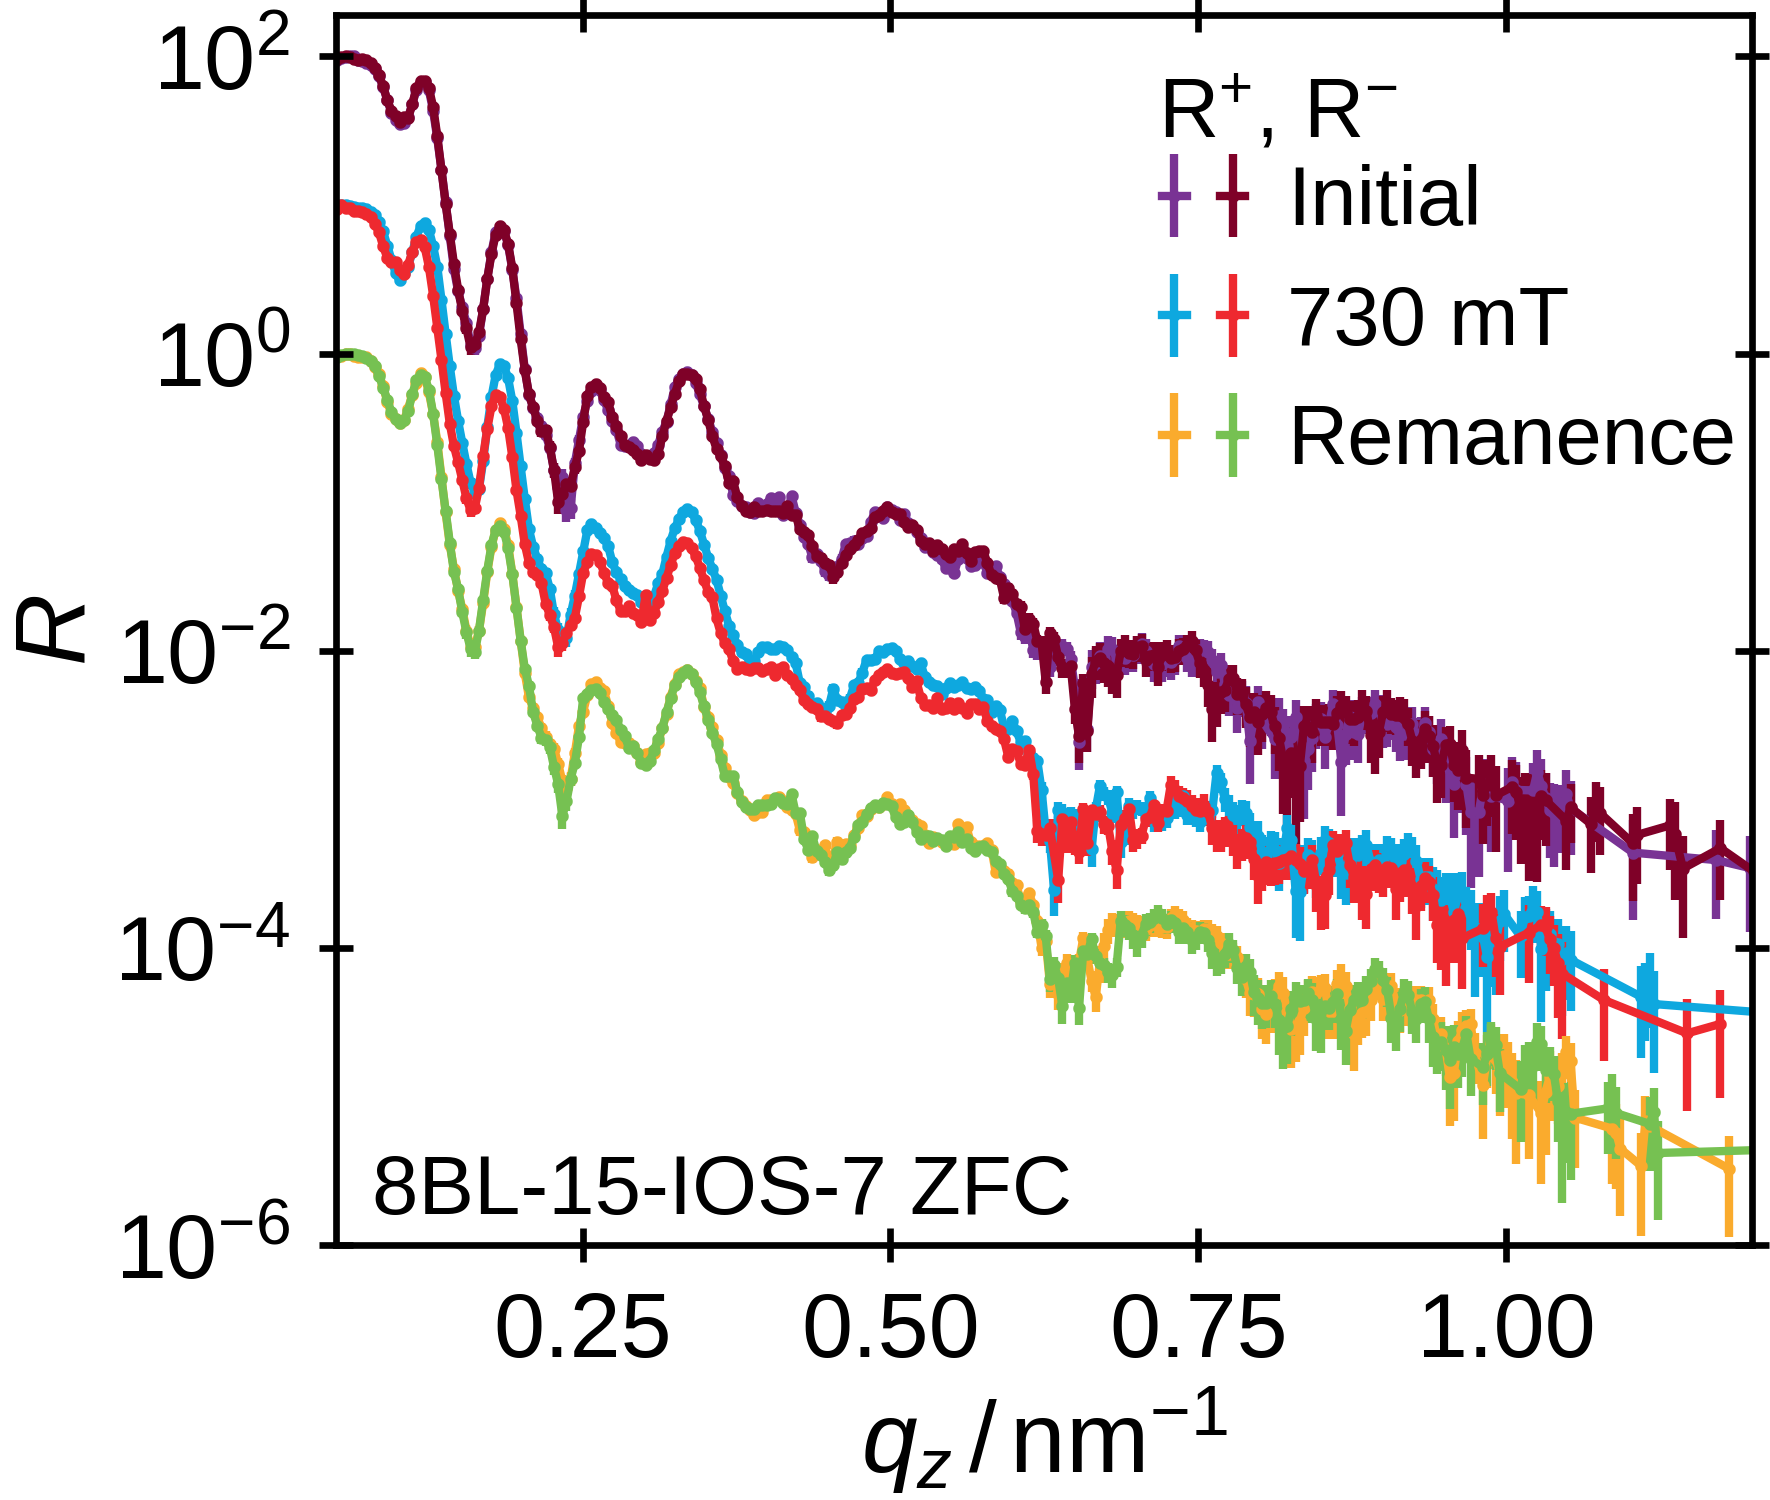
\includegraphics{looselyPackedNP_VerticalStructure_8BL-15-IOS-7_PNR_ZFC30K}
    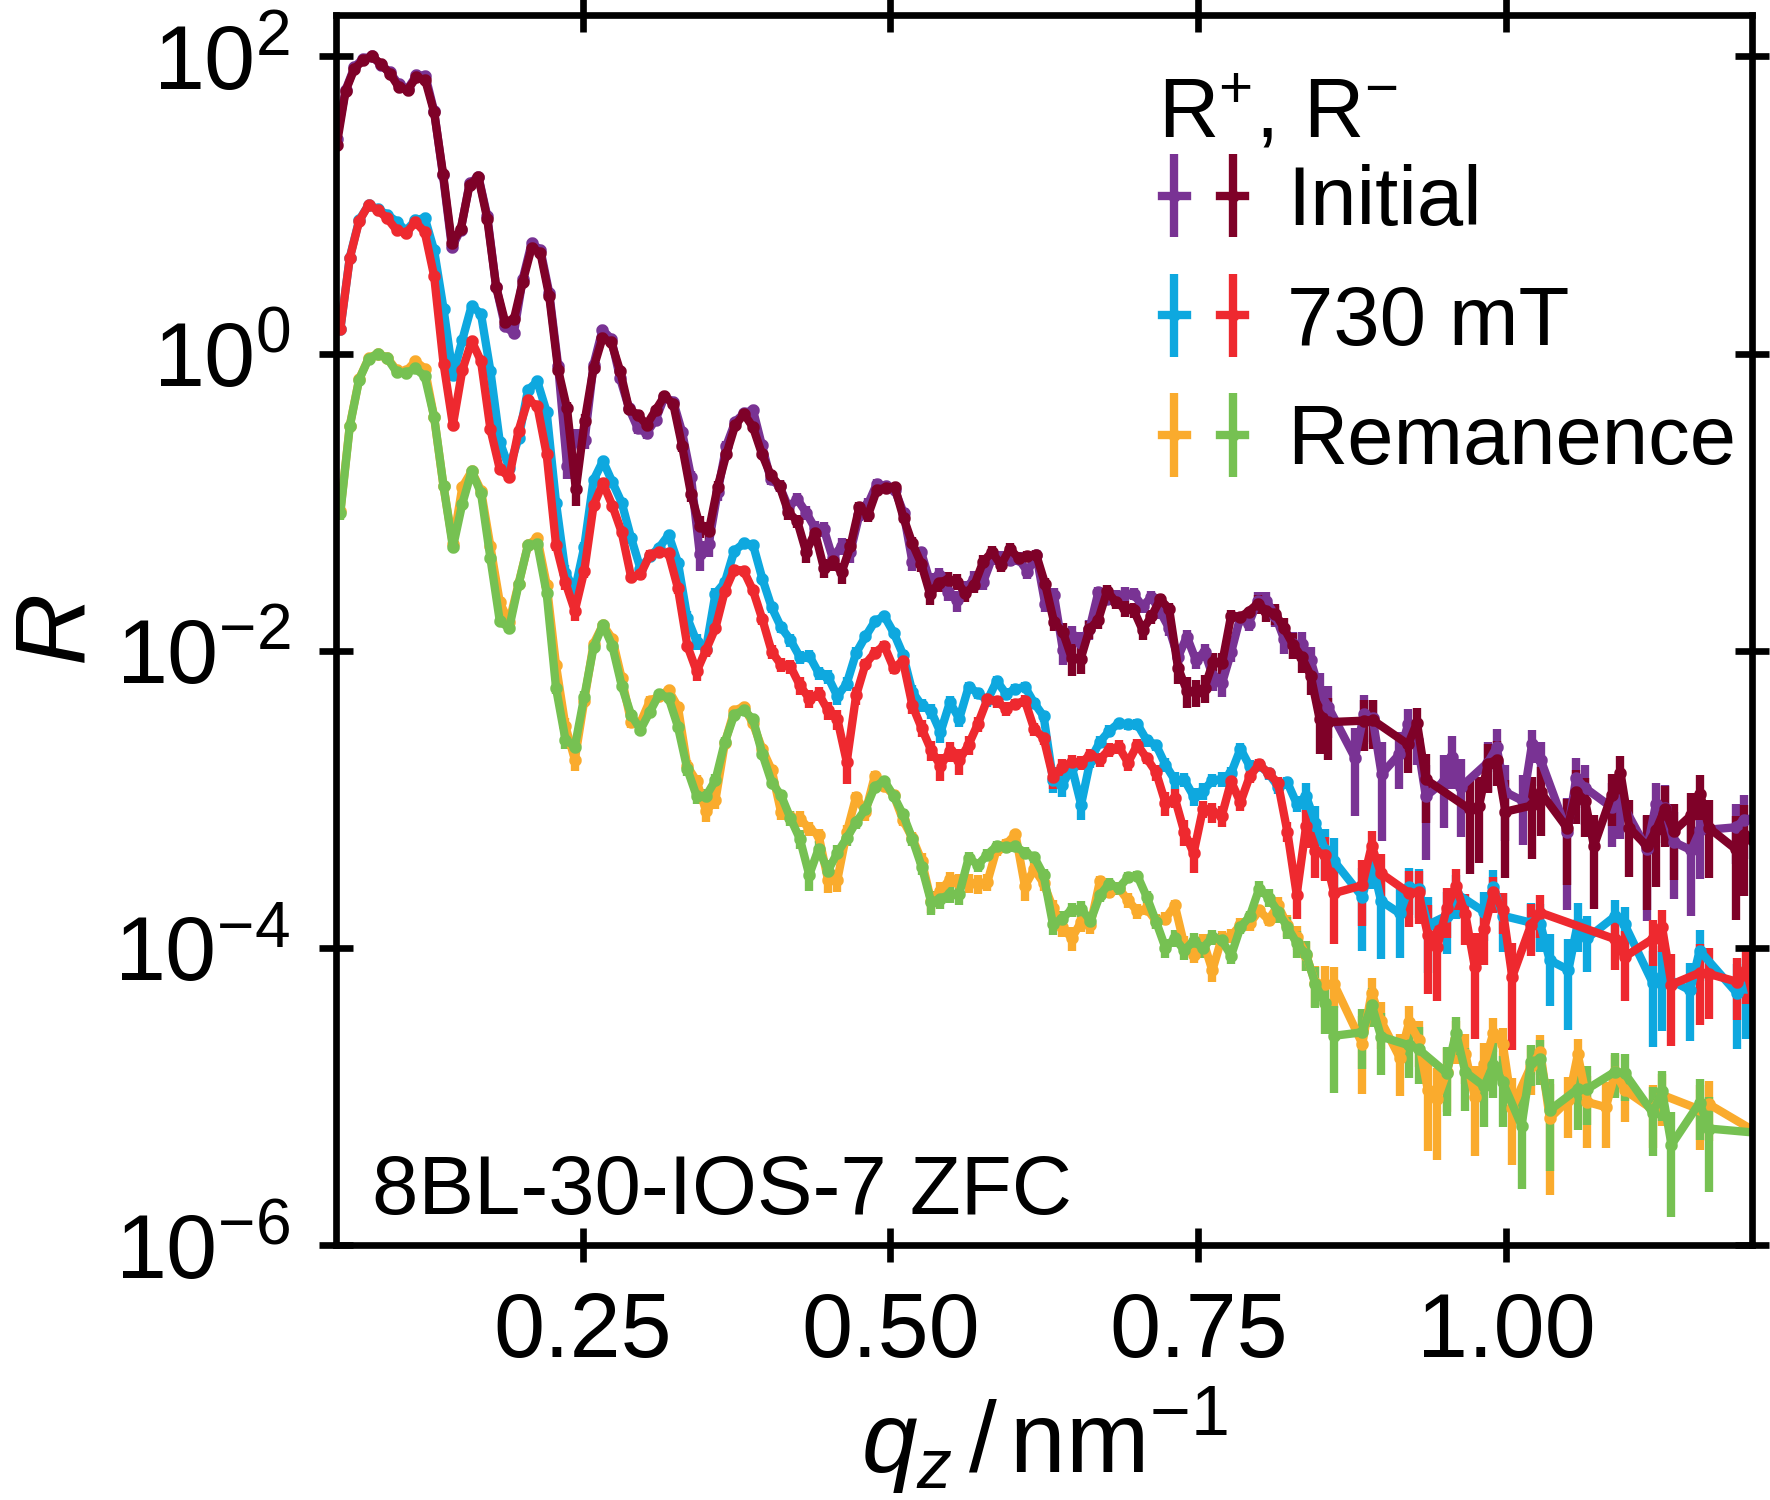
\includegraphics{looselyPackedNP_VerticalStructure_8BL-30-IOS-7_PNR_ZFC30K}
    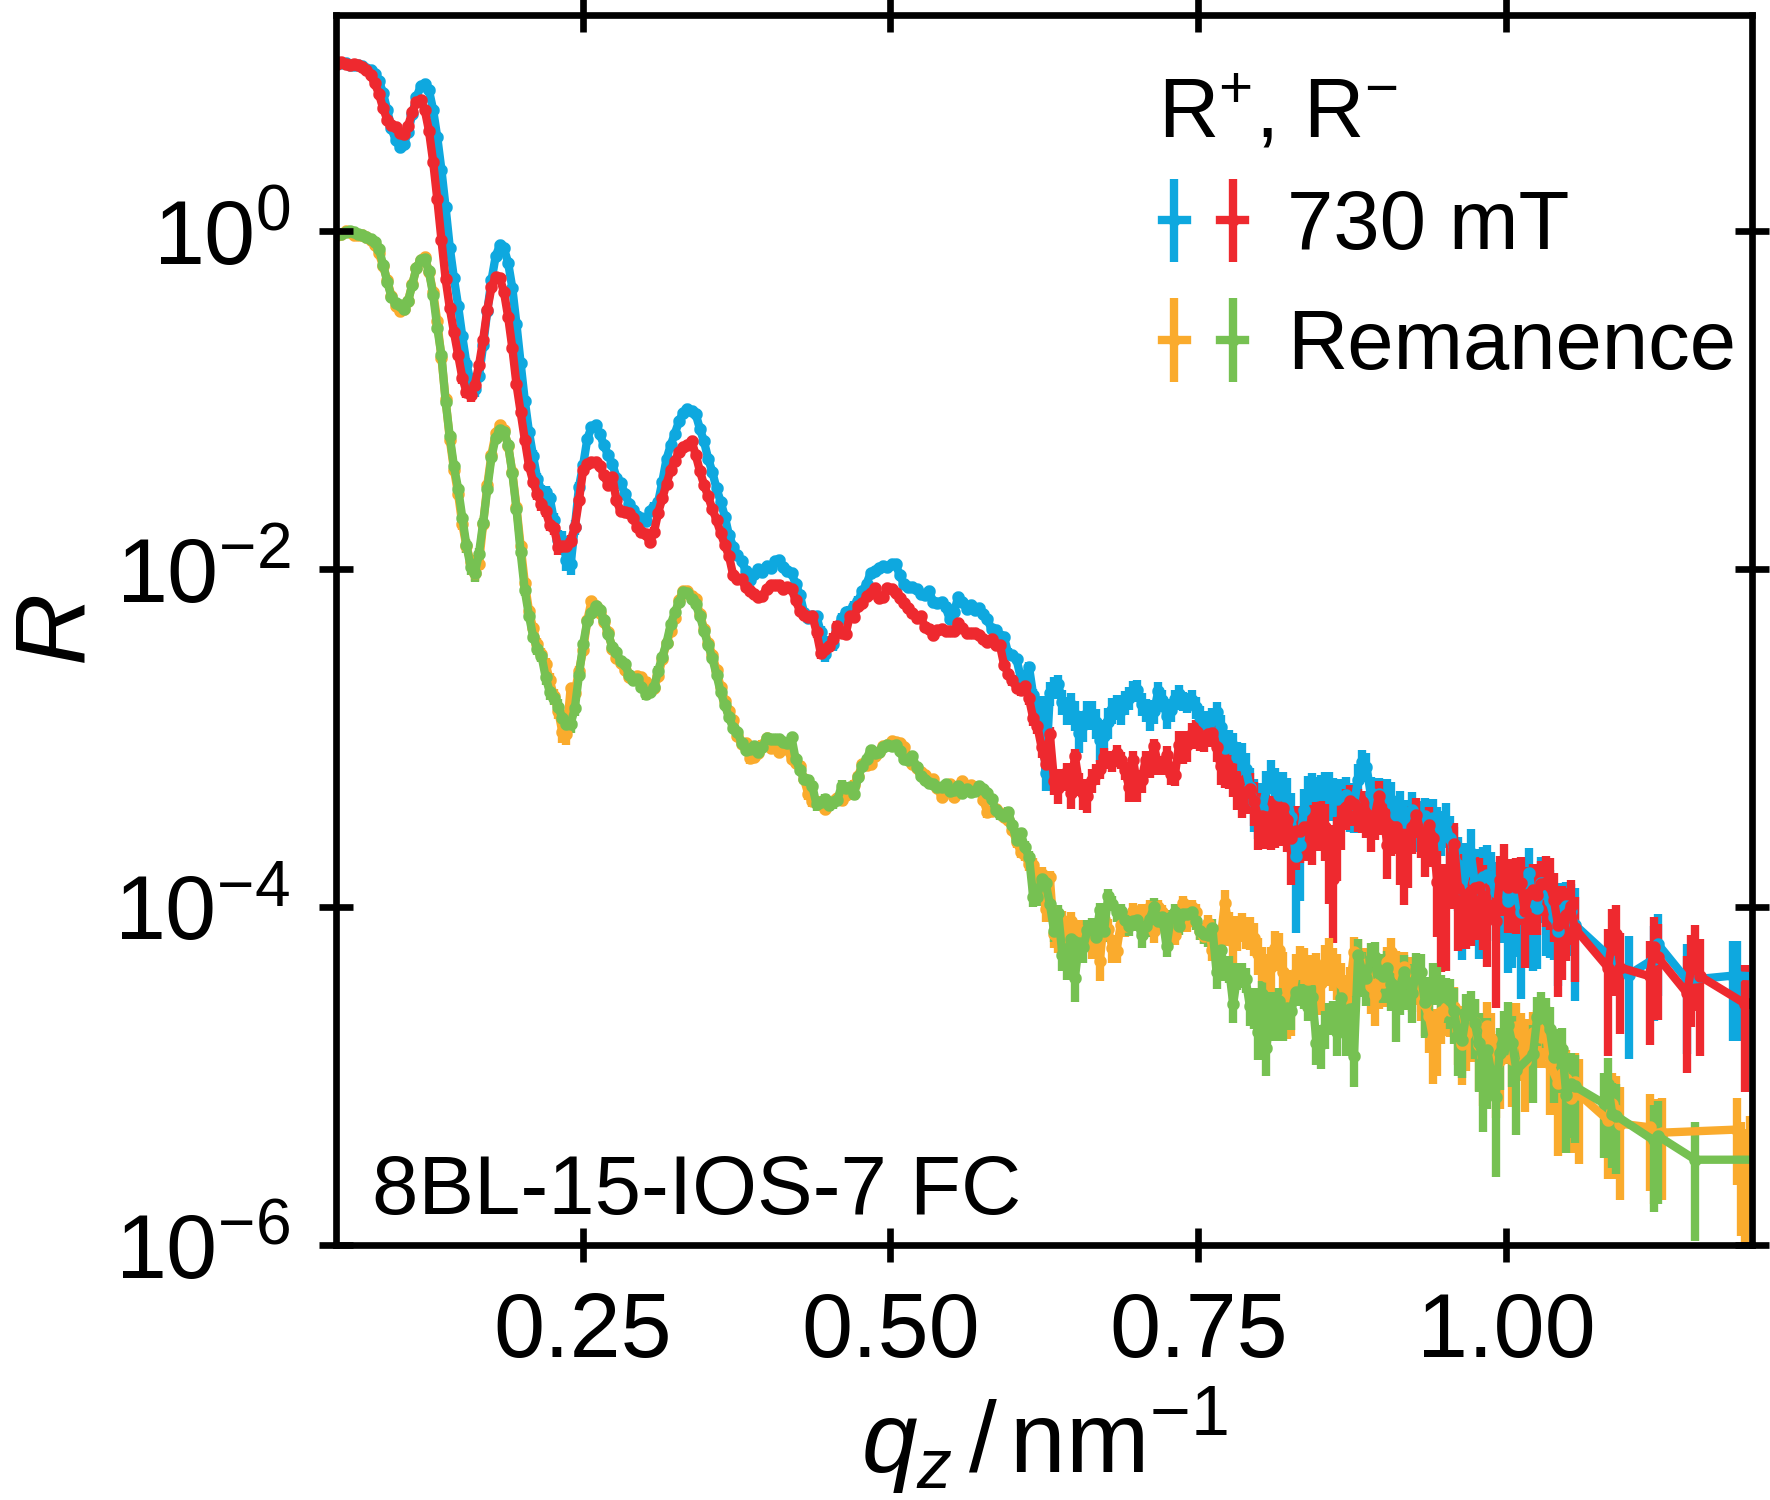
\includegraphics{looselyPackedNP_VerticalStructure_8BL-15-IOS-7_PNR_FC30K}
    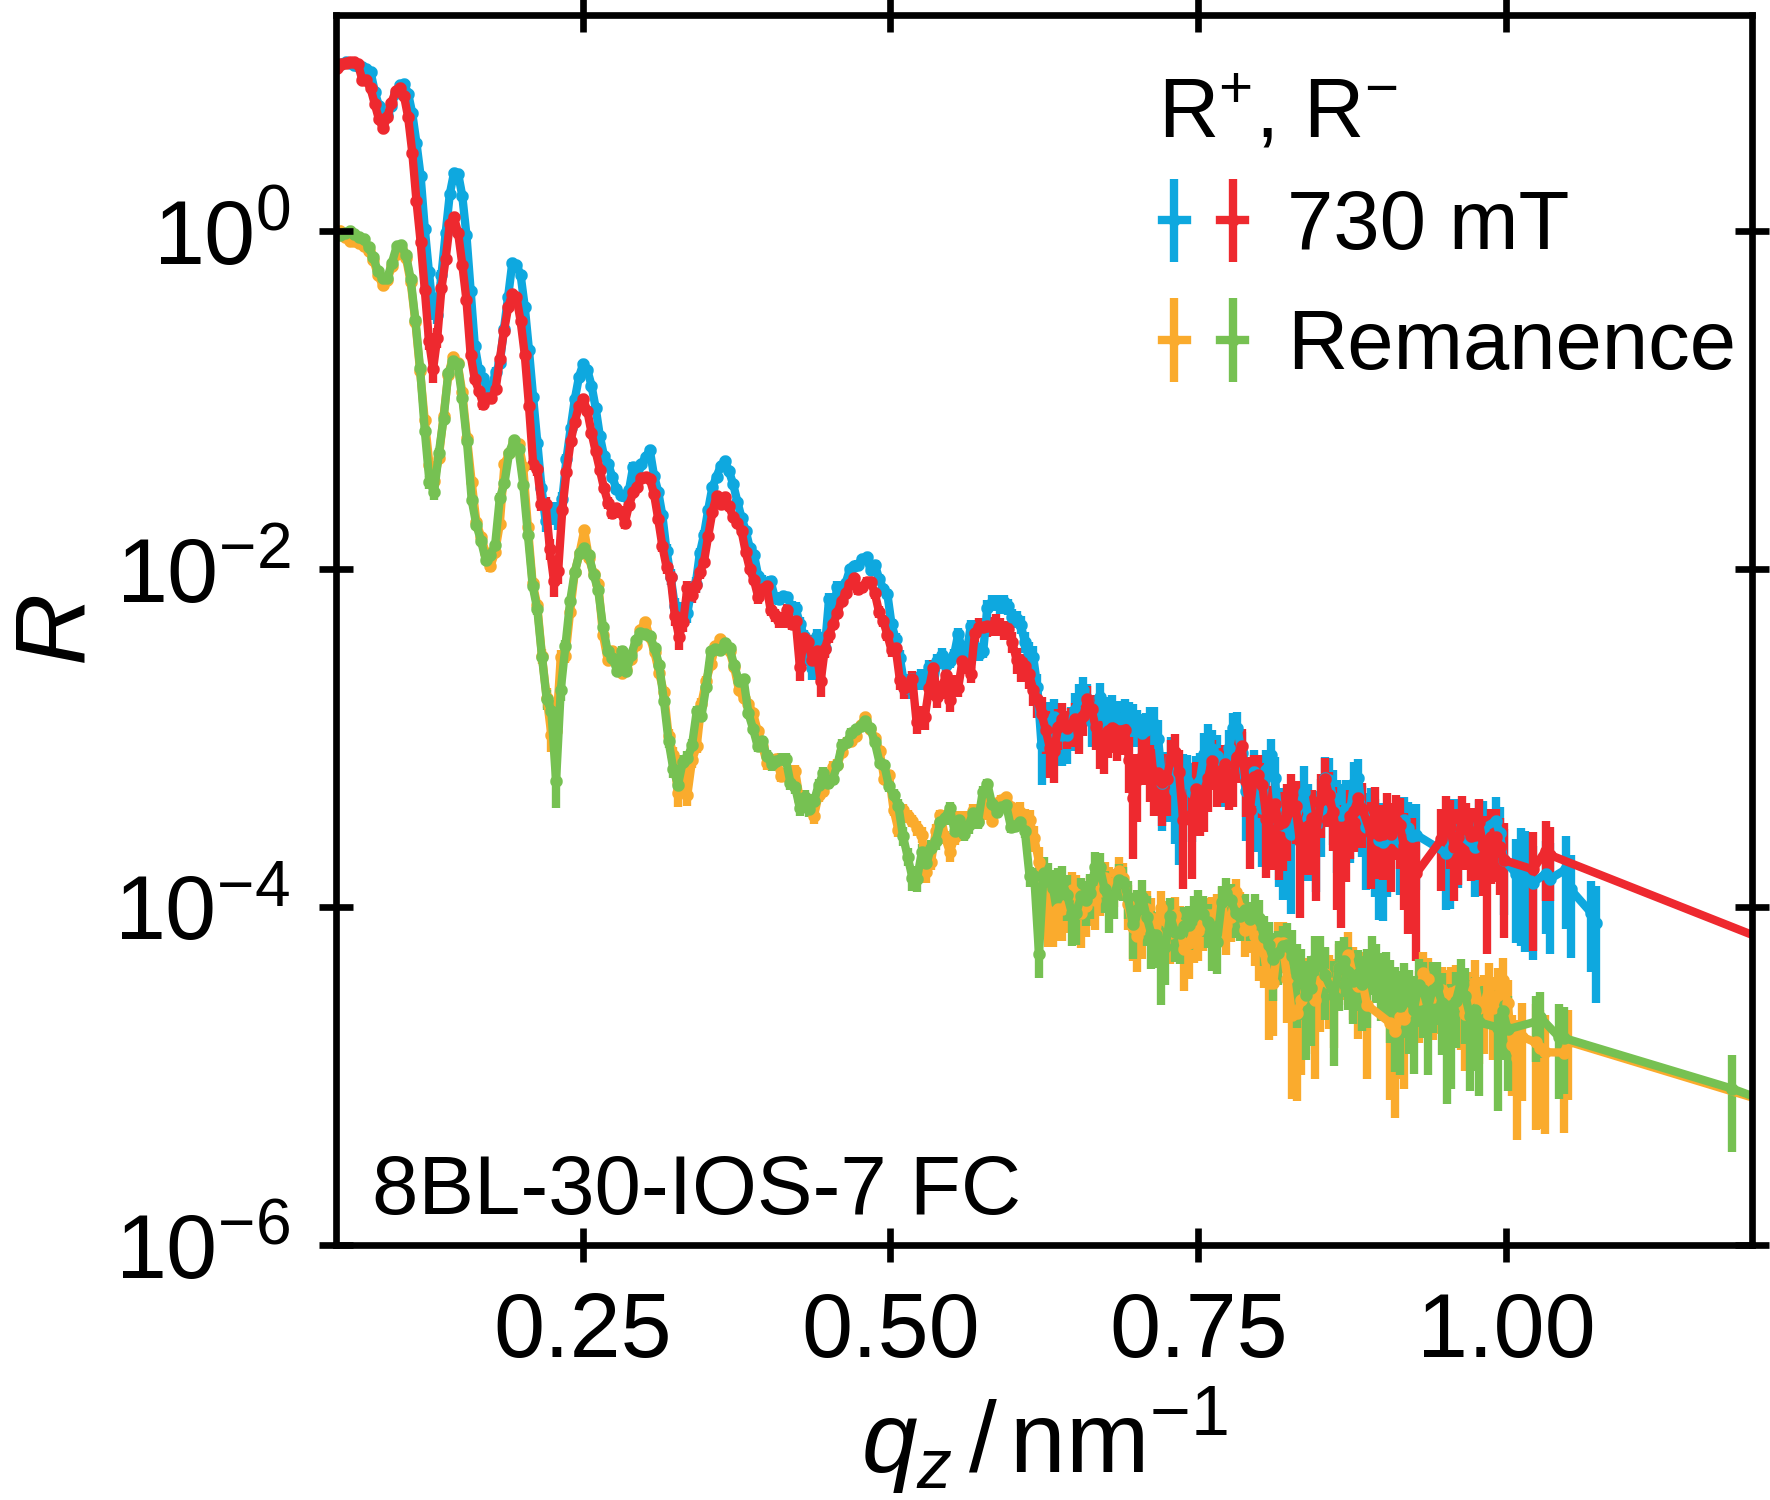
\includegraphics{looselyPackedNP_VerticalStructure_8BL-30-IOS-7_PNR_FC30K}
    \caption{\label{fig:looselyPackedNP:bilayer:pnr:8BL-x-IOS7}PNR of 8BL-15-IOS-7 (left) and 8BL-30-IOS-7 (right) after zero-field cooling (upper) and field cooling (lower).}
  \end{figure}
\end{document}